\documentclass[main.tex]{subfiles}

\begin{document}
\section{Spracovanie dát}

\subsection{Scraping prieskumov agentúry FOCUS}
Na účely tohto projektu potrebujeme mať značnú históriu volebných prieskumov v jednotnom formáte.
Nakoľko však agentúra FOCUS nezverejňuje s každým prieskumom jednotný .xlsx alebo .csv súbor a rovnako na svojej stranke nemá zverejnené všetky prieskumy, ktoré kedy vykonala, tak je táto úloha obzvlášť problematická.
Väčšina vykonaných prieskumov je však k dispozícií vo formáte .pdf v štýle reportu (Press release). Javí sa, že FOCUS pri týchto reportoch udržuje jednotný formát v priebehu rokov, čo využijeme na extrakciu dát z nich.

Súčasťou každého takéhoto .pdf súboru je aj samotný prieskum, napríklad:

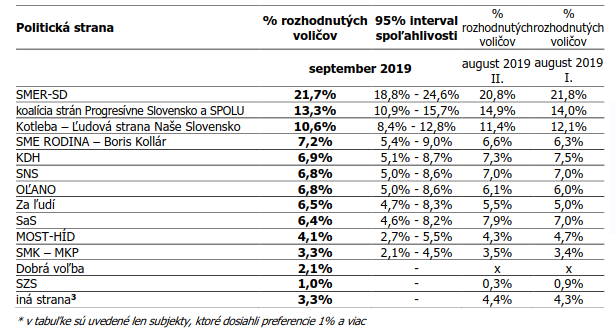
\includegraphics[width=0.8\textwidth]{figs/priklad-focus-prieskumu.png}

Automatizovaného sťahovanie z webu sme vykonali pomocou Python knižnice \href{https://github.com/SeleniumHQ/Selenium}{Selenium}, ktorá vie interagovať s webovým prehliadačom ako bežný používateľ. Pomocou iteratívneho odosielania query do prehliadača vo forme: "focus prieskum volby {month} {year}" + " filetype:pdf" sme stiahli prvý result vo forme .pdf súboru. Avšak ak v danom mesiaci nebol uskutočnený prieskum, resp. prvý nájdený .pdf súbor obsahoval niečo iné, stiahli sme zbytočný súbor. Takéto situácie sme museli následne ručne identifikovať a odstrániť. 

Nakoniec sa nám úspešne podarilo takýchto reportov získať 127. 

Ďalej sme tabuľky z reportov agentúry FOCUS automatizovane extrahovali na účel vytvorenia jednotného .csv súboru. Použili sme Python knižnicu \href{https://github.com/DS4SD/docling}{Docling}, pomocou ktorej sme prekonvertovali tabuľky z .pdf do pd.DataFrame, spojili a exportovali do jednotného \verb*|data/raw/polls/focus_polls.csv|.

Tento proces nebol úplne priamočiary. Názvy politických strán sa extrahovali veľmi nekonzistentne.
Takisto viaceré politické strany menili meno v priebehu rokov, takže bolo potrebné manuálne vytvoriť mapper, ktorý tieto názvy zjednotil. Ďalej bolo potreba niektoré záznamy aj manuálne opraviť, keďže strany s dlhším názvom (v reporte zabrali dva riadky tabuľky) sa duplikovali v našom extrahovanom datasete.

Po týchto všetkých úkonoch sme už mali jednotný formát dát, ktorý zachytával prieskumy z mnohých mesiacov.

\end{document}
